\section{Access to Computational Resources}

By the end of the workshop we hope you're thinking one or more of the following:

\begin{itemize}
\item I'm interested in dabbling some more during my day-job!
\item How do I access a Linux box like the one I've been using in the workshop -
I \emph{really} don't want the hassle of setting this all up myself!
\item I'm hooked! I \emph{really} want to get down and dirty with NGS data! What
computational resources do I need, what do I have access to and how do I access
them?
\end{itemize}

We're ecstatic you're thinking this way and want to help guide you! However, lets
take this one step at a time.

The quickest way to dabble is to use a clone of the operating system (OS) you've
been using during this workshop. That means you'll have hassle-free access to a
plethora of pre-installed, pre-configured bioinformatics tools. You could even set it
up to contain a copy of all the workshop data and handouts etc to go through the
hands-on practicals in your own time!

We have created an image file (approx. 10 GBytes in size) of the NGS Training OS for you to
use as you wish:
\\\\
%\url{https://swift.rc.nectar.org.au:8888/v1/AUTH_809/NGSImage/NGSTrainingV1.0.vdi}
\url{https://swift.rc.nectar.org.au:8888/v1/AUTH_33065ff5c34a4652aa2fefb292b3195a/VMs/NGSTrainingV1.2.1.vdi}
\\\\
We would advise one of the following two approaches for making use of it:

\begin{itemize}
\item Import it into VirtualBox to setup a virtual machine (VM) on your own
computer.
\item Instantiate a VM on the NeCTAR Research Cloud.
\end{itemize}

\subsection{Setting up a VM using VirtualBox}
This approach requires the least amount of mind-bending to get up and running.
However, you will need to install some software. If you do not have
administrator access or your system administrator is slow or unwilling to
install the software, you may find using the NeCTAR Research Cloud to be viable
alternative.

This approach will use, at most, the computational resources available on
your own computer. If you are analysing non-microbial organisms or performing
\textit{de novo} assemblies, you may find these resources are insufficient. If this is the
case, you really should speak to someone from IT support at your institution or
get in touch with a bioinformatician for advise.

The software you need is VirtualBox, a freely available, Open Source
virtualisation product from Oracle (\url{https://www.virtualbox.org/}). This
software essentially allows you to run an operating system (the guest OS) within
another (the host OS). VirtualBox is available for several different host OSes
including MS Windows, OS X, Linux and Solaris
(\url{https://www.virtualbox.org/wiki/Downloads}). Once VirtualBox is installed
on your host OS, you can then install a guest OS inside VirtualBox. VirtualBox
supports a lot of different OSes
(\url{https://www.virtualbox.org/wiki/Guest_OSes}).

Here are the steps to setting up a VM in VirtualBox with our image file:
\begin{enumerate}
  \item Download and install VirtualBox for your OS: 
  \url{https://www.virtualbox.org/wiki/Downloads}
  \item Start VirtualBox and click New to start the Create New Virtual Machine wizard
  \item Give the VM a useful name like ``NGS Training'' and choose Linux and
  either Ubuntu or Ubuntu (64-bit) as the OS Type
  \item Give the VM access to a reasonable amount of the host Oses memory. i.e.
  somewhere near the top of the green. If this value is $<$ 2000 MB, you are
  likely to have insufficient memory for your NGS data analysis needs.
  \item For the virtual hard disk, select ``Use existing hard disk'' and browse
  to and select the \texttt{NGSTrainingV1.2.1.vdi} file you downloaded.
  \item Confirm remaining settings
  \item Select the ``NGS Training'' VM and click Start to boot he machine.
  \item Once booted, log into the VM as either \texttt{ubuntu} (a sudoer user;
  i.e. has admin rights) or as \texttt{ngstrainee} (a regular unprivileged
  user). See table below for passwords.
\end{enumerate}


\subsection{Setting up a VM using the NeCTAR Research Cloud}
All Australian researchers, who are members of an institution which subscribes
to the Australian Access Federation (AAF; \url{http://www.aaf.edu.au/}), have
access to a small amount of computing resources (2 CPU's and 8 GBytes RAM) on
the NeCTAR Research Cloud (\url{http://nectar.org.au/research-cloud}).

\subsubsection{Login to the NeCTAR Research Cloud Dashboard}
The online dashboard is a graphical interface for administering (creating,
deleting, rebooting etc) your virtual machines (VMs) on the NeCTAR research
cloud.

\begin{enumerate}
  \item Go to the dashboard: \url{http://dashboard.rc.nectar.org.au}
  \item When you see the following page, click the ``Log In" button:
  \begin{figure}[H]
    \centering
    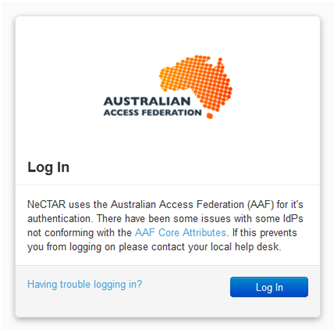
\includegraphics[scale=0.5]{handout/nectar/aaf_login.png}
    \caption{\label{fig:aaf_login}}
  \end{figure}
  \item At the following screen, simply choose your institution from the
  dropdown box and click ``Select". Now follow the on screen prompts and enter
  your regular institutional login details.
  \begin{figure}[H]
    \centering
    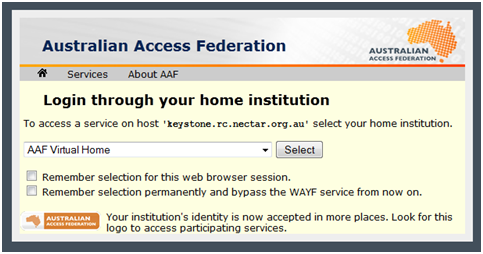
\includegraphics[scale=0.5]{handout/nectar/aaf_home_institute.png}
    \caption{\label{fig:aaf_home_institute}}
  \end{figure}
  \item If you see the following screen, congratulations, you have
  successfully logged into the NeCTAR Research Cloud dashboard!
  \begin{figure}[H]
    \centering
    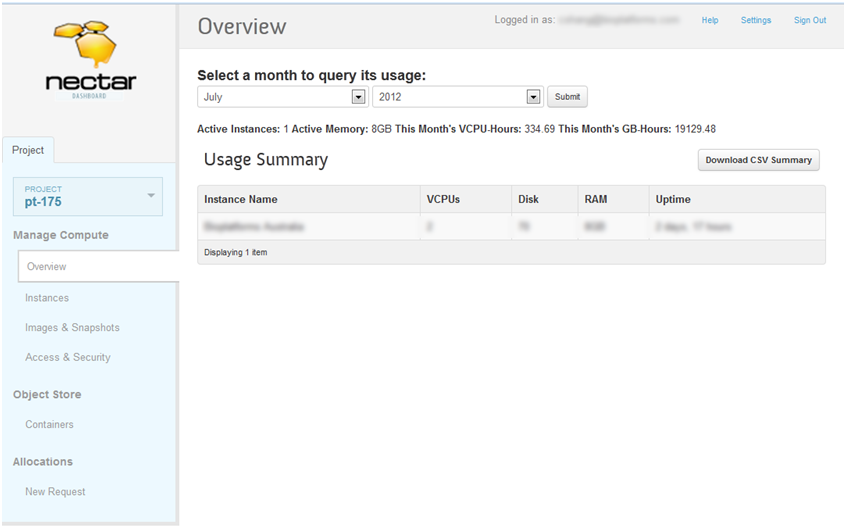
\includegraphics[scale=0.5]{handout/nectar/dashboard_overview.png}
    \caption{\label{fig:dashboard_overview}}
  \end{figure}
\end{enumerate}

\subsubsection{Instantiating Your Own VM}
We will now show you how to instantiate the ``NGS Training'' image using your
own personal cloud allocation.

\begin{enumerate}
  \item In the NeCTAR Research Cloud dashboard, click ``Images \& Snapshots''
  to list all the publicly available images from which you can instantiate a
  VM. Under ``Snapshots" Click the ``Launch" button for the latest version of the
  ``NGSTraining" snapshot:
  \begin{figure}[H]
    \centering
    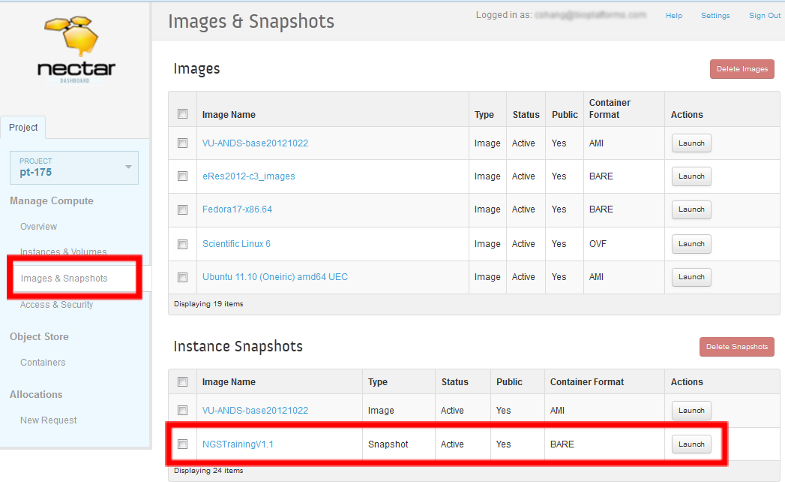
\includegraphics[scale=0.5]{handout/nectar/dashboard_snapshots.png}
    \caption{\label{fig:dashboard_snapshots}}
  \end{figure}
  \item You will now see a ``Launch Instances'' window where you are required to
  enter some details about how you want the VM to be setup before clicking
  ``Launch Instance".
  In the ``Launch Instances'' pop-up frame choose the following settings:
  \begin{description}
  \item[Server Name] A human readable name for your convenience. e.g. ``My NGS VM''
  \item[Flavor] The resources you want to allocate to this VM. I suggest a
  Medium sized VM (2 CPUs and 8 GBytes RAM). This will use all your personal
  allocation, but anything less will probably be insufficient. You could request
  a new allocation of resources if you want to instantiate a larger VM with more
  memory.
  \item[Security Groups] Select SSH.
  \end{description}
  \item Click the ``Launch Instance'' button
  \begin{figure}[H]
    \centering
    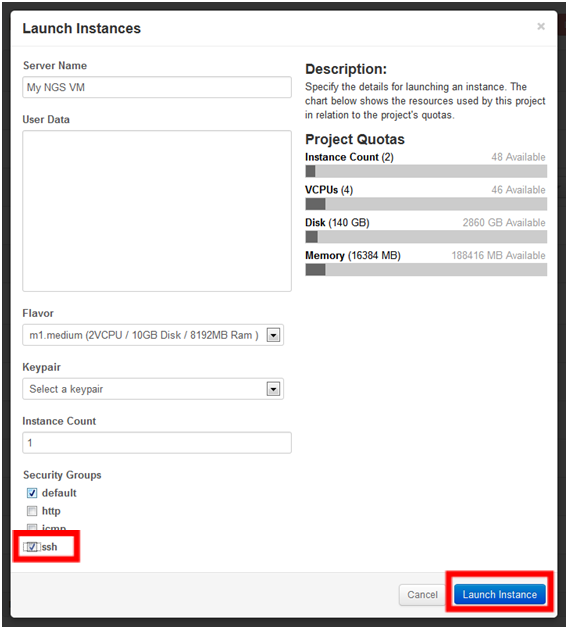
\includegraphics[scale=0.5]{handout/nectar/dashboard_launch.png}
    \caption{\label{fig:dashboard_launch}}
  \end{figure}
  \item You will be taken to the ``Instances" page and you will see the
  ``Status" and ``Task" column for your new VM is ``Building" and ``Spawning". Once
  the ``IP Address" cell is populated, take a note of it as you will need it for
  configuring the NX Client later on.
  \begin{figure}[H]
    \centering
    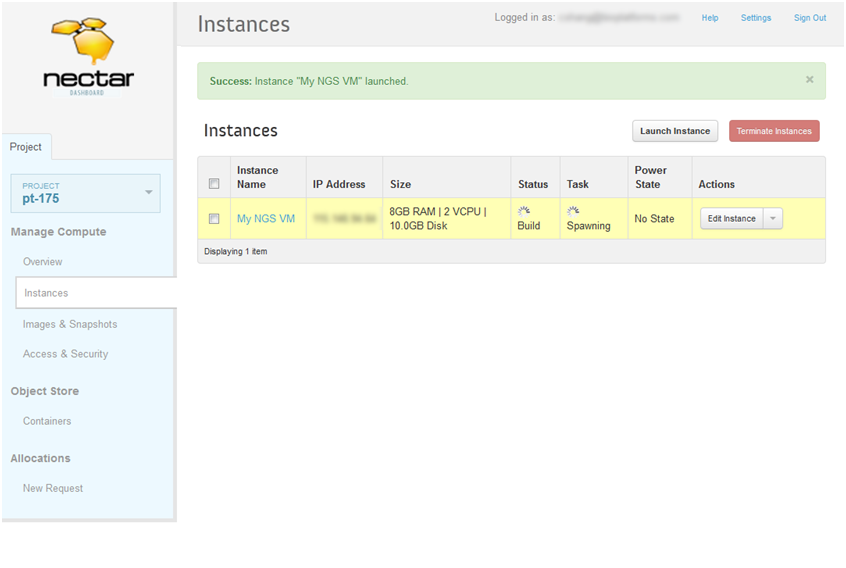
\includegraphics[scale=0.5]{handout/nectar/dashboard_instance_building.png}
    \caption{\label{fig:dashboard_instance_building}}
  \end{figure}
  \item Once the Status and Task for the VM change to ``Active and ``None"
  respectively, your VM is powered up and is configuring itself.
  Congratulations, you have now instantiated a Virtual Machine! If you try to
  connect to the VM too quickly, you might not be successful. The OS may still
  be configuring itself, so give it a few minutes to finish before continuing.
  \begin{figure}[H]
    \centering
    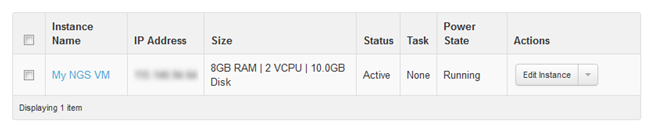
\includegraphics[scale=0.5]{handout/nectar/dashboard_instance_running.png}
    \caption{\label{fig:dashboard_instance_running}}
  \end{figure}
\end{enumerate}

\subsubsection{VM Stuck Building and Spawning}
Sometimes, the cloud experiences a ``hiccup" and a newly instantiated VM will get
stuck in the ``Build" and ``Spawning" state (step 3) for more than a few minutes.
This can be rectified by terminating the instance and creating a new VM from
scratch:
\begin{enumerate}
  \item Selecting ``Terminate Instance" under the ``Edit Instance" dropdown box:
  \begin{figure}[H]
    \centering
    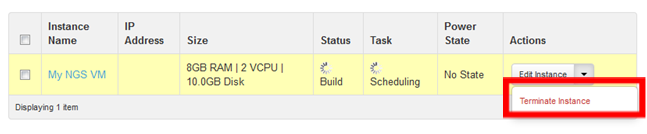
\includegraphics[scale=0.5]{handout/nectar/dashboard_terminate_stuck_instance.png}
    \caption{\label{fig:dashboard_terminate_stuck_instance}}
  \end{figure}
  \item Go back to step 1 of ``Instantiating Your Own VM" and create the VM from scratch:
\end{enumerate}
  

\subsection{Remote Desktop with the NoMachine NX Client}
During the workshop you were using the free NX client from NoMachine
(\url{http://www.nomachine.com/}) to provide a remote desktop-like connection to
VMs running on the NeCTAR Research Cloud. Therefore, we provide information on how to
setup your local computer to connect to the VM you just instantiated in the steps
above.

We assume that:
\begin{itemize}
\item You have administrator rights on your local computer for installing
software.
\end{itemize}

\subsubsection{NoMachine NX Client Installing}
We show you instructions below for the MS Windows version of the NX Client, but
procedures for other supported OSes (Linux, Mac OSX and Solaris) should be very
similar.
\begin{enumerate}
  \item Go to the NoMachine download page: \url{http://www.nomachine.com/download.php}
  \item Click the download icon next to the NX Client for Windows:
  \begin{figure}[H]
    \centering
    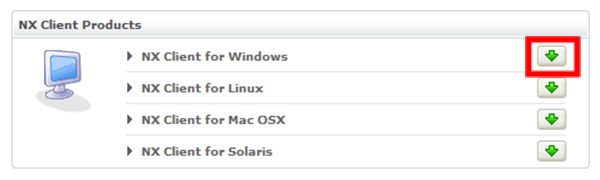
\includegraphics[scale=0.5]{nx_client/download.png}
    \caption{\label{fig:nx_download}}
  \end{figure}
  \item On the "NX Client for Windows" page, click the "Download package" button:
  \begin{figure}[H]
    \centering
    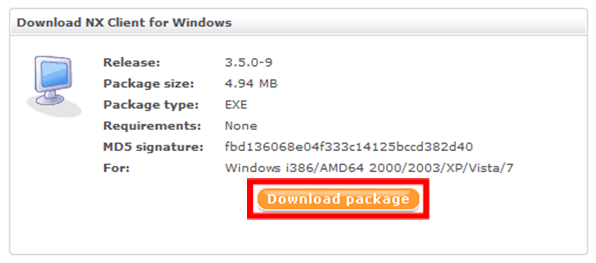
\includegraphics[scale=0.5]{nx_client/download_package.png}
    \caption{\label{fig:nx_download_package}}
  \end{figure}
  \item Run the file you just downloaded (accepting defaults is fine)
  \item Congratulations, you just installed the NoMachine NX Client!
\end{enumerate}

\subsection{NoMachine NX Client Configuration}
Now we have the NoMachine NX Client installed, we need to configure a new NX
"session" which will point to the VM we instantiated in the NeCTAR Research
Cloud.

We assume that:
\begin{itemize}
\item You know the IP address of the VM you want to remote desktop into.
\end{itemize}

\begin{enumerate}
  \item Start the NX Connection Wizard and click "Next" to advance to the
  "Session" settings page.
  \begin{figure}[H]
    \centering
    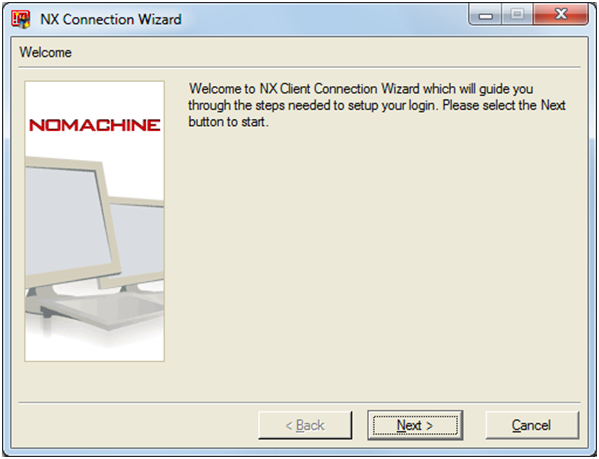
\includegraphics[scale=0.5]{nx_client/start_wizard.png}
    \caption{\label{fig:nx_start_wizard}}
  \end{figure}
  \item On the "Sessions" settings page enter the following details:
  \begin{description}
  \item[Session] A memorable name so you know which VM this session is pointing
  at. You could use the same name you chose for the VM you instantiated earlier
  e.g. "NGS Training".
  \item[Host] Enter the IP address of the VM you instantiated on the NeCTAR
  Research Cloud.
  \begin{figure}[H]
    \centering
    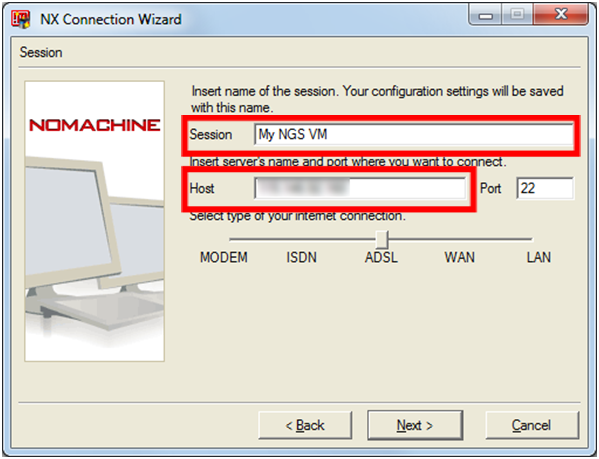
\includegraphics[scale=0.5]{nx_client/session_configuration.png}
    \caption{\label{fig:nx_session_configuration}}
  \end{figure}
  \end{description}
  \item Click "Next" to advance to the "Desktop" settings page. You should use the
  "Unix GNOME" setting.
  \begin{figure}[H]
    \centering
    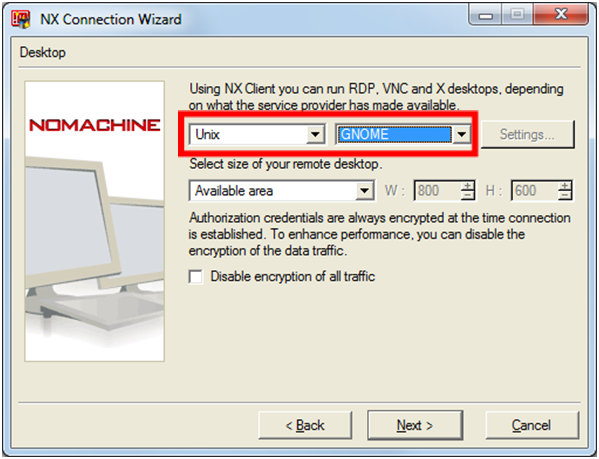
\includegraphics[scale=0.5]{nx_client/desktop_type.png}
    \caption{\label{fig:nx_desktop_type}}
  \end{figure}
  \item Click "Next" and "Finish" to complete the wizard.
\end{enumerate}

\subsection{Connecting to a VM}
If you just completed the NX Connection Wizard described above, the wizard
should have opened the NX Client window. If not, run the "NX Client". You will
be presented with a window like this:
\begin{figure}[H]
  \centering
  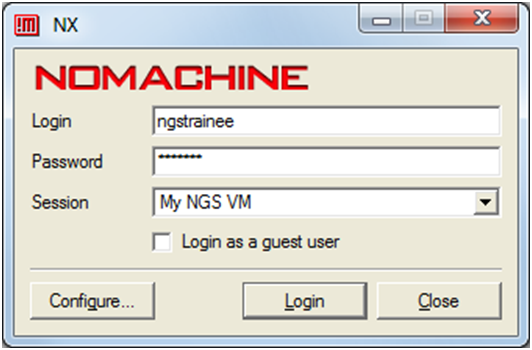
\includegraphics[scale=0.5]{nx_client/login.png}
  \caption{\label{fig:nx_login}}
\end{figure}

The "Login" and "Password" boxes in the NX Client are for user accounts setup on
the VM. By default our image, from which you instantiated your VM, has two
preconfigured users:
\begin{figure}[H]
  \centering
  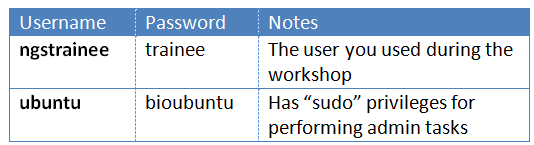
\includegraphics[scale=0.5]{nx_client/usernames_passwords.png}
  \caption{\label{fig:nx_usernames_passwords}}
\end{figure}

Unless you know what you are doing, we suggest you use the \texttt{ngstrainee}
user account details to initiate an NX connection to your VM. In less than a
minute, you should see an NX Window showing the desktop of your VM:
\begin{figure}[H]
  \centering
  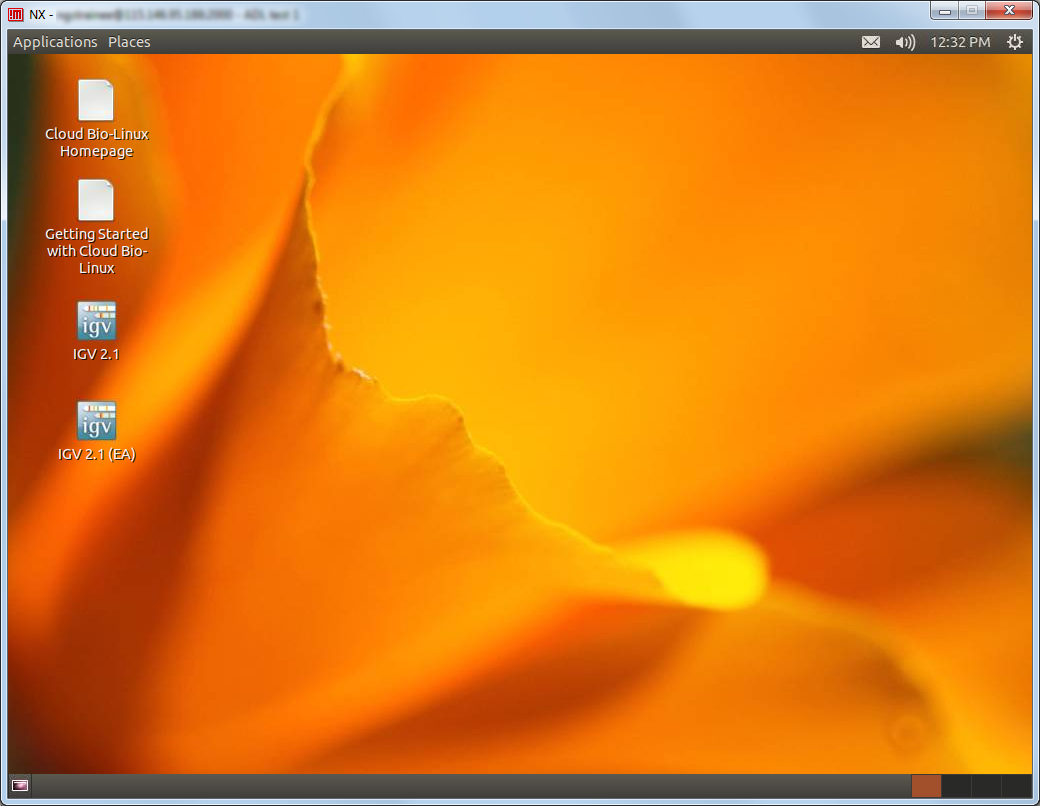
\includegraphics[width=0.8\textwidth]{nx_client/connected.png}
  \caption{\label{fig:nx_connected}}
\end{figure}

\subsection{NX Connection Failure}
In the event that you don't get the NX Window with your VM's desktop displaying
inside it. The most common errors are:
\begin{itemize}
\item You failed to select the "ssh" security group when instantiating the VM.
You'll need to terminate the instance and create a new VM from scratch
\item You failed to select "Unix GNOME" when you configured the NX Client
session. You'll need to reconfigure the session using the NX Client
\item Your institutions firewall blocks TCP port 22. You may need to request this
port to be opened by your local network team or configure the NX client to use a
proxy server.
\end{itemize}

\subsection{Advanced Configuration}
In the session configuration, you can configure the size of the NX Window in
which the desktop of the VM is drawn:
\begin{figure}[H]
  \centering
  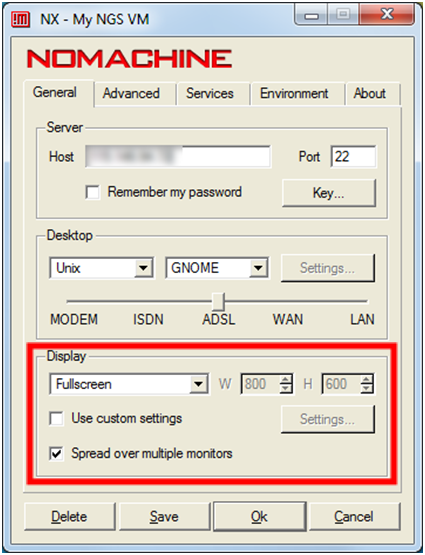
\includegraphics[scale=0.5]{nx_client/advanced_display.png}
  \caption{\label{fig:nx_advanced_display}}
\end{figure}

This can be useful if you want to:
\begin{itemize}
\item Have the NX Window occupy the entire screen, without window decorations.
This is often desirable if you wish to "hide" the host OS from the person
sitting at the computer running the NX Client.
\item Have the NX Window spread over multiple monitors.
\end{itemize}

